% Created 2019-06-02 Sun 01:03
% Intended LaTeX compiler: pdflatex
\documentclass[11pt]{article}
\usepackage[utf8]{inputenc}
\usepackage[T1]{fontenc}
\usepackage{graphicx}
\usepackage{grffile}
\usepackage{longtable}
\usepackage{wrapfig}
\usepackage{rotating}
\usepackage[normalem]{ulem}
\usepackage{amsmath}
\usepackage{textcomp}
\usepackage{amssymb}
\usepackage{capt-of}
\usepackage{hyperref}
\usepackage{minted}
\usepackage{parskip}
\author{Marc-André Chénier}
\date{\today}
\title{}
\hypersetup{
 pdfauthor={Marc-André Chénier},
 pdftitle={},
 pdfkeywords={},
 pdfsubject={},
 pdfcreator={Emacs 26.2 (Org mode 9.1.9)}, 
 pdflang={English}}
\begin{document}

\tableofcontents


\section{Question 3}
\label{sec:org2addb33}
The contour probability for \(H_{0}:\theta_{0}=0.25\) is obtained with
two computational approaches solving the same problem: measuring the
area under the beta posterior density curve with limits defined such
that \(p(\theta|y) > p(\theta_{0}|y)\). When \(\theta_{\text{0}}\) is less than the
mode of the posterior density, this area corresponds to \(P(\theta_{0}
< \theta < \delta)\), with density \(p(\delta | y)=p(\theta_{0})\). In this
scenario, the complement \(p_{b}\) of the probability \(P(\theta_{0} <
\theta < \delta)\) can be interpreted as the counterpart of a two-sided
p-value. This is the contour probability.

In the first approach, we simply look for \(\delta\) such that
\((P(\theta_0|y) - P(\delta|y))^2=0\). This is accomplished with the
numerical optimization \textbf{R} program \emph{optimize}. Again assuming
\(\theta_{0}\) to be the lower limit of integration, the complement of
\(p_{b}\) is then obtained from:

\begin{align}
\label{eq:org201972e}
\begin{split}
P(\theta_{0} < \theta < \delta) =& \int_{\theta_{0}}^{\delta}
P(\theta | y) d\theta \\
=&\int_{\theta_{0}}^{\delta}\frac{1}
{\operatorname{Beta}(\bar{\alpha}, \bar{\beta})} \theta^{\bar{\alpha}-1} 
(1 - \theta)^{\bar{\beta} - 1} \\
=& F(\delta | y) - F(\theta_{0} | y)
\end{split}
\end{align}

with the \textbf{R} digital table for the beta cumulative distribution
\(F\). In the second approach, we first obtain the mode \(\bar{\theta}\)
of the posterior beta density with
\(\frac{\bar{\alpha}-1}{\bar{\alpha} + \bar{\beta}-2}\). Then, for the
case where \(\theta_{0}\) is less than \(\bar{\theta}\), we search for
\(\delta\) in the interval \([\bar{\theta}, 1]\) such that \(P(\theta_{0} |
y)=P(\delta | y)\). This is accomplished with the \textbf{R} program
\emph{uniroot}. Once \(\delta\) is obtained, the complement of the contour
probability \(p_{b}\) is measured by following Equation \ref{eq:org201972e}. Both
approaches give return the same contour probabilities.

As in Questions 2 and 3, we give dose 0 an informative conjugate prior
with \(\alpha=y-1=29\) and \(\beta=n-y-1=193\). The other doses are given
vague beta priors with \(\alpha=1\) and \(\beta=1\) which correspond to a
uniform distribution with support from 0 to 1. In Table \ref{tab:org382fe79},
the contour probabilities are presented for each dose. The probability
at dose 500 couldn't converge because 1 is the maximum of the beta
distribution and the posterior mode as a value of 1. Convergence could
have be obtained with an informative prior. For every dose, the
probability of the true \(\theta\) being 0.25 is less than 0.05. Thus,
we conclude that the \(H_0\) is implausible and reject it. Remarkably
with dose 0, we would have kept \(H_{0}\) had the prior been
non-informative (i.e. \(p_b=0.68\)).

\begin{table}[H]
\caption{\label{tab:org382fe79}
Contour probabilities for \(H_0\):\(\theta_0=0.25\) per dose level}
\centering
\begin{tabular}{cccccc}
\hline
\textbf{Dose} & \textbf{\(\theta_0\)} & \textbf{\(\delta\)} & \textbf{p\(_{\text{b}}\)} & \textbf{1 - p\(_{\text{b}}\)} & \textbf{Obj.}\\
0 & 0.25 & 0.137 & 0.001 & 0.999 & 0\\
62.5 & 0.25 & 0.140 & 0.035 & 0.965 & 0\\
125 & 0.25 & 0.947 & 0.000 & 1.000 & 0\\
250 & 0.25 & 1.000 & 0.000 & 1.000 & 0\\
500 & 0.25 & 1.000 & 0.000 & 1.000 & NA\\
\hline
\end{tabular}
\end{table}

In Figure \ref{fig:orgce72a9a}, the complement of the contour probabilities are
illustrated for each dosage. These are coloured in grey and the
plotted curves are the posterior beta distributions.

\begin{figure}[H]
\centering
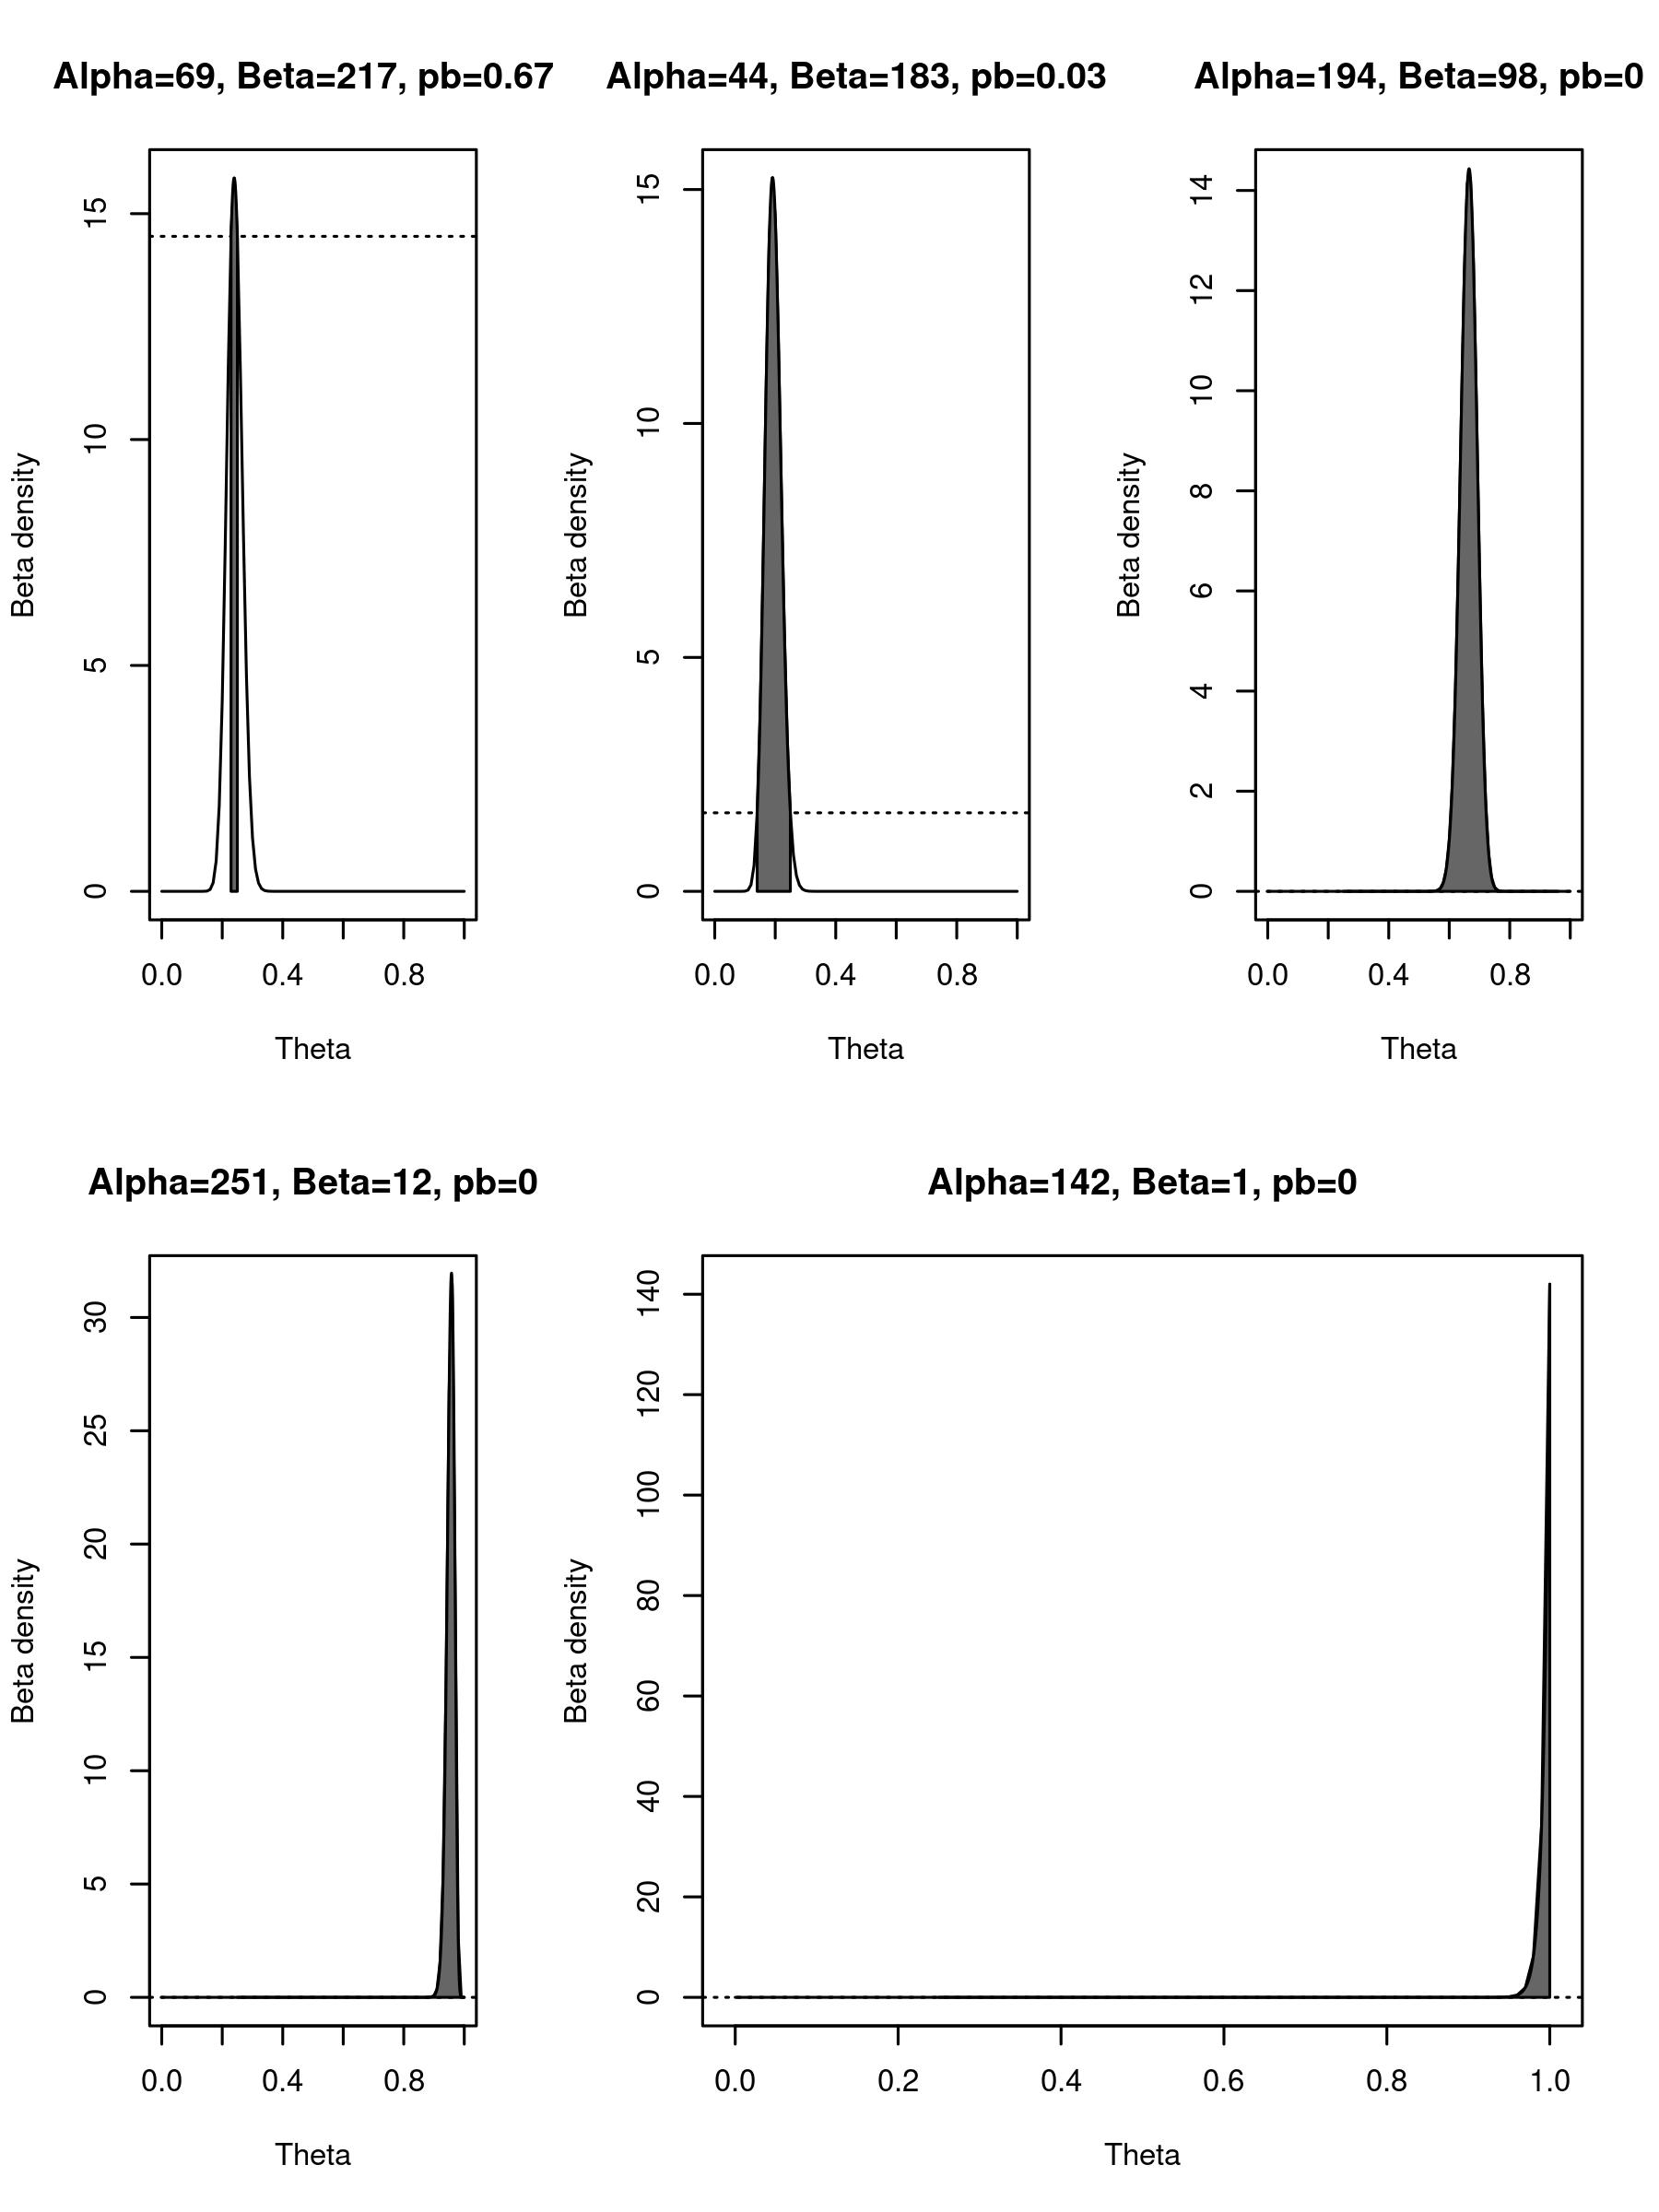
\includegraphics[width=.5\textwidth]{./q2_contourplots.jpg}
\caption{\label{fig:orgce72a9a}
Contour probability plots per dose}
\end{figure}

\section{Question 10}
\label{sec:orgdcecd46}
Our goal here is to find the dosage associated with an increase of
0.01 in excess risk \(q\) of foetus malformation. It is useful to
reformulate the question in order to clarify the problem and its
solution.

The excess risk \(q\) is associated with a probability of malformation
\(P(d^{*})\) by:

\begin{equation}
P(d^{*})=q(1-P(0)) + P(0)
\end{equation}

where \(P(0)\) is the prevalence of foetus malformation at a dose 0 of
diglyme. The logit of \(P(d)\), the probability of malformation at a
given dose, can be estimated with the linear model \(\alpha + \beta*
\mathrm{dose}\). As such, the dose we are looking for can be deduced
with simple algebra from

\begin{equation}
\label{eq:org4c19ae1}
\mathrm{dose}=\mathrm{BMD}=\frac{\operatorname{logit}(P(d^{*})) 
- \alpha}{\beta}
\end{equation}

provided we have estimates for \(\alpha\) and \(\beta\). This dose is
called the benchmark dose (BMD). From Question 3, we posess samples
from the posterior distributions of \(\beta\) and \(\alpha\). Thus, we can
not only furnish a point estimate of the BMD, but also express its
uncertainty with a certitude interval. Only, as the dose variable is
standardized, Equation \ref{eq:org4c19ae1} becomes

\begin{equation}
\mathrm{BMD}=\left(\frac{\operatorname{logit}(P(d^{*})) - \alpha}
{\beta}\right) s_{\mathrm{dose}} + \operatorname{avg}(\mathrm{dose})
\end{equation}

where \(s\) and \(\operatorname{avg}\) respectively designate the standard
deviation and mean of the dose covariate.

Assuming that the prevalence at dose 0, \(P(0)\), is known and obtained
from the proportion in the provided table (i.e. 0.238), we get a mean
BMD of 32.17 with a \(95\%\) equal-tails certitude interval of 20.53 to
42.79.
\end{document}